
\section{LDR Sensor}

\subsection{Introduction}
A Light Dependent Resistor (LDR) is a type of photoresistor 
whose resistance changes based on the intensity of light falling on it.
In this experiment, the LDR is used as an analog input sensor that allows
ambient light levels to automatically control the brightness of an LED.
As the surrounding light increases or decreases, the voltage across the LDR
changes accordingly.

This changing voltage is read by the microcontroller through one of its
analog input pins. The input value is then mapped to a range suitable
for Pulse Width Modulation (PWM), which is used to adjust the LED brightness.
In low light, the LED becomes brighter, and in bright light, it dims.
This setup demonstrates how sensors like LDRs can be used to creat
e responsive and automatic lighting systems based on environmental conditions.
\subsection{Procedure}
1. Gathered an STM32F103C6 blue pill board, LDR, LED, $220\Omega$ resistor, breadboard, and jumper wires.

2. Placed the LDR on the breadboard. Connected one side to 3.3V and the other side to PB1 (analog input) and also to GND through a fixed resistor to form a voltage divider.

3. Connected the LED's anode to PB0 (PWM output) through a $220\Omega$ resistor, and the cathode to GND.

4. Verified all connections were secure and correct.

5. Uploaded the code via PlatformIO. The LED brightness changed automatically in response to ambient light levels detected by the LDR.
\subsection{Diagram}
\begin{figure}[htbp]
    \centering
    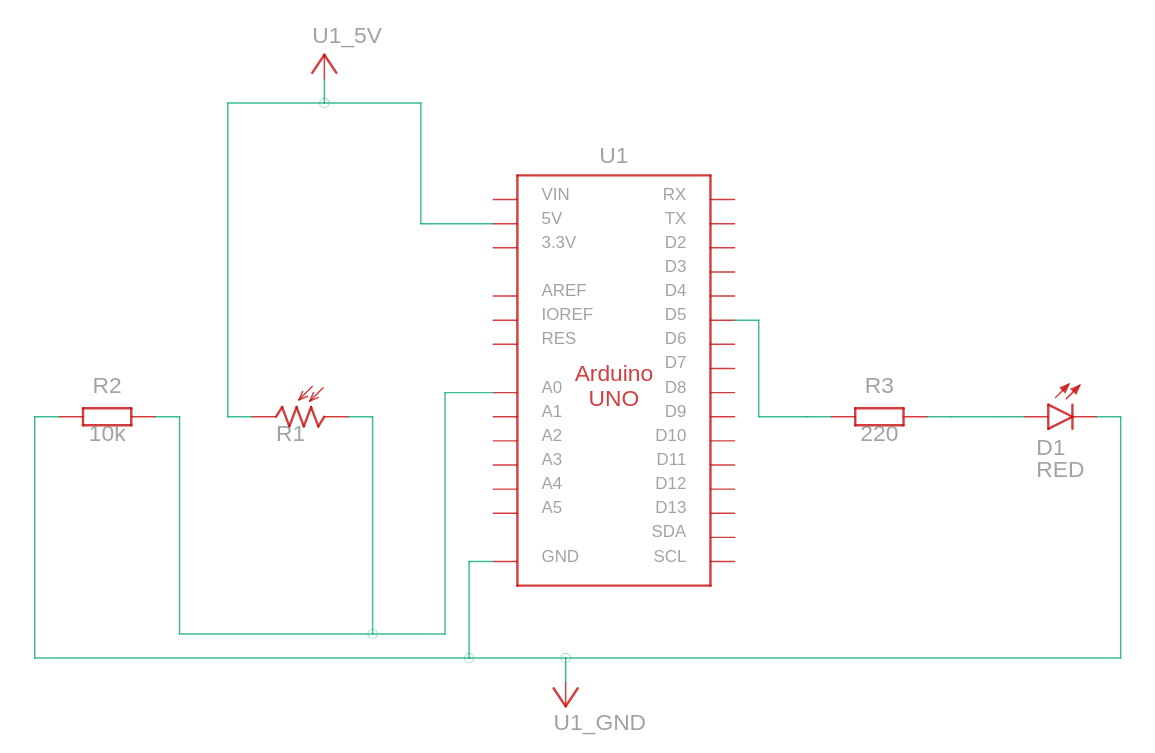
\includegraphics[width=0.6\textwidth]{img/ldr.png}
    \caption{Schematic diagram of the circuit using Arduino in TinkerCAD}\label{fig:ldrr}
\end{figure}

\subsection{Source Code}

\begin{code}
\caption{LED control using LDR sensor}
\begin{minted}[frame=single, linenos]{cpp}
#include <Arduino.h>
#define LED PB0
#define LDR PB1
void setup() {
  pinMode(LED, OUTPUT);
  pinMode(LDR, INPUT);
}

void loop() {
  int value = analogRead(LDR);
  value = map(value, 0, 1023, 255, 0);
  analogWrite(LED, value);
  delay(500);
}
\end{minted}
  \label{code:LDR}
\end{code}

\subsection{Discussion}
In this experiment, I successfully used an LDR sensor to automatically
control the brightness of an LED through PWM using an STM32 microcontroller
and the Arduino framework. The code read the analog voltage from the LDR,
mapped it inversely to a 0–255 range, and used analogWrite()
to adjust the LED's brightness accordingly.
As expected, the LED became brighter in low light and dimmer in bright light
, confirming that the analog input was correctly processed
and translated into a PWM output.

The results matched the intended behavior,
showing a clear and consistent change in LED brightness based on ambient
light levels detected by the LDR.
This demonstrated the practical application of analog-to-digital
conversion and pulse-width modulation in responsive lighting control.

Through this experiment, I learned how to read and interpret
sensor data, apply mapping for output control, and use PWM to adjust
LED intensity dynamically. It also reinforced my understanding of sensor
integration and the interaction between hardware and software
to create automated systems.

